\documentclass{beamer}

% rubber: module pdftex

%\mode<presentation>
%{
%  \usetheme{Boadilla}
%}

\usepackage[finnish]{babel}
\usepackage[utf8]{inputenc}
\usepackage{times}
\usepackage[T1]{fontenc}
\usepackage{amsmath}
\setbeamertemplate{navigation symbols}{}

\title{Järjestämisalgoritmit}

\subtitle{Superlaskenta kotitietokoneella}

\author{Laura Leppänen}

\date{19. maaliskuuta, 2012}

\begin{document}

\begin{frame}
\titlepage
\end{frame}

\section{Arkkitehtuurin kertausta}

\begin{frame}{Arkkitehtuurin kertausta}{Suorittimet}
  \begin{figure}
    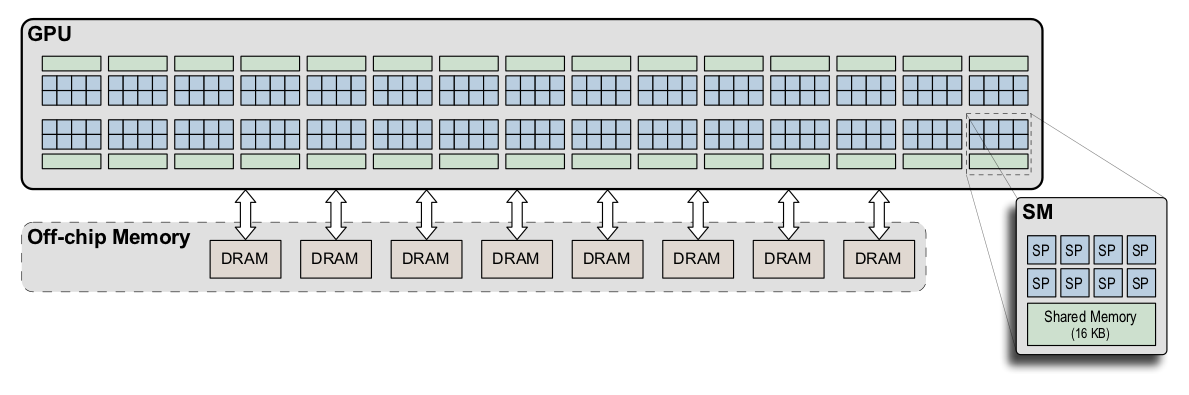
\includegraphics[scale=0.25]{geforce_gtx280.png}
    \caption{Geforce GTX 280}
  \end{figure}

  \begin{itemize}
  \item
    Useita moniprosessoreita (\emph{streaming multiprocessor}), joilla useita ytimiä.
  \item
    Kommunikaatio moniprosessorien välillä hidasta.
    % Tapahtuu tyypillisesti globaalin muistin kautta.
  \end{itemize}
\end{frame}

\begin{frame}{Arkkitehtuurin kertausta}{Säikeiden suoritus}
    \begin{itemize}
    \item
    Säikeet jaetaan lohkoihin ja lohkot 32 säikeen nippuihin (\emph{warp}).
    % Nipun koko riippunee näytönohjainkortista.
    \item
      Samaan nippuun kuuluvat säikeet suorittavat samaa käskyä samaan aikaan.
    \item
      Optimaalisessa tilanteessa kaikki saman nipun säikeet valitsevat saman suorituspolun.
    \item
      Yhtäaikaisia säikeitä tarvitaan paljon (tuhansia).
    \end{itemize}
\end{frame}

\begin{frame}{Arkkitehtuurin kertausta}{Muistit}
  \begin{figure}
    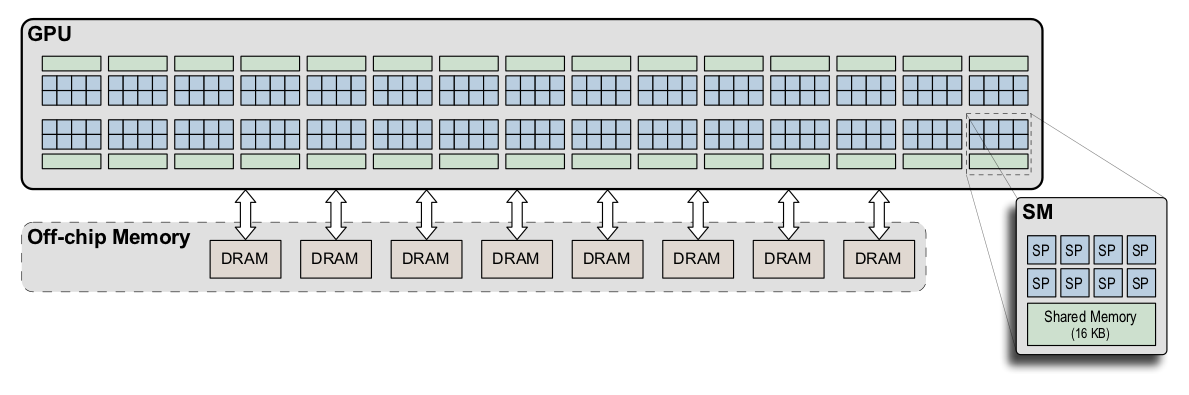
\includegraphics[scale=0.25]{geforce_gtx280.png}
  \end{figure}
    \begin{itemize}
    \item
      Jokaisella prosessorilla pieni määrä rekistereitä.
      % Eli ytimellä
    \item
      Moniprosessorin ytimien kesken jaettu muisti (nopeaa).
    \item
      Globaali muisti (hidasta).
    \item
      Isäntäjärjestelmän muisti (erittäin hidasta).
    \item
      Viittaukset useisiin rinnakkaisiin paikkoihin muistissa voidaan yhdistää yhdeksi luku- tai kirjoitusoperaatioksi.
    \end{itemize}
\end{frame}

\begin{frame}{Arkkitehtuurin kertausta}{Työnjako (CPU ja GPU)}
    \begin{itemize}
    \item
      Isäntäsovellus (sarjallinen) isäntäarkkitehtuurilla.
    \item
      CUDA-ytimet (\emph{kernel}) näytönohjaimella.
    \item
      Datan siirtäminen isäntäarkkitehtuurilta näytönohjaimelle hyvin hidasta. \\ $\Rightarrow$ Datan järjestäminen voi usein olla nopeampaa tehdä isäntäjärjestelmässä GPU:n sijaan.
    \item
      Uudemmissa CUDA Toolkitin versioissa mahdollisuus allokoida isäntäjärjestelmän muistia suoraan CUDA-ytimien käyttöön.
    \end{itemize}
\end{frame}

\section{Järjestämisalgoritmit}

% Pitäisikö olla jokin yleisesittely ongelmasta?

\begin{frame}{CUDA-järjestämisalgoritmit}{Yleistä}
    \begin{itemize}
    \item
      Tehokkaimmat toteutukset kantalukujärjestämisalgoritmeja (\emph{radix sort})
    \item
      Ainakin yksi merge sort -toteutus.
    \item
      Järjestämisverkkoihin perustuvat algoritmit, jotka on erityisesti suunniteltu rinnakkaisille arkkitehtuureille.
    \item
      Yhtäkään erityisen tehokasta quicksort-toteutusta ei näytä olevan.
    \end{itemize}
\end{frame}

\section{Bitoninen järjestäminen}

\begin{frame}{Bitoninen järjestäminen}{(Batcher 1967)}
    \begin{itemize}
    \item
      Vertailuun perustuva algoritmi.
    \item
      Järjestää alkiot vakiotyötilassa (\emph{in place}).
    \item
      Perustuu järjestämisverkon käyttöön. \\ $\Rightarrow$ Suunnattu nimenomaan rinnakkaisille arkkitehtuureille.
    \item
      Tarvittavien vertailuoperaatioiden määrä riippuu ainoastaan syötteen pituudesta ($n$), ei esimerkiksi alkioiden jakaumasta.
    \end{itemize}
\end{frame}

\begin{frame}{Bitoninen järjestäminen}{Bitoninen järjestämisverkko}
    \begin{figure}
        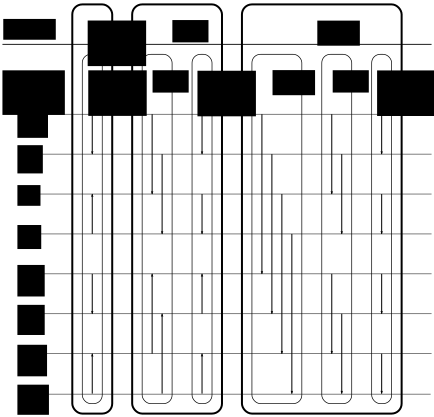
\includegraphics[scale=0.5]{bitonic.pdf}
        \caption{Bitoninen järjestämisverkko $n = 8 = 2^3$ alkiolle}
    \end{figure}
    % Selitä:
    % * syötelangat
    % * vertailuoperaattorit ja nuolten suunnan merkitys
    \begin{itemize}
        \item
          Verkossa $k$ vaihetta, kun $n = 2^k$.
          % Ja jokaisessa vaiheessa p on p kpl askeleita.
    \end{itemize}
\end{frame}

\begin{frame}{Bitoninen järjestäminen}{Bitoninen järjestämisverkko}
    \begin{figure}
        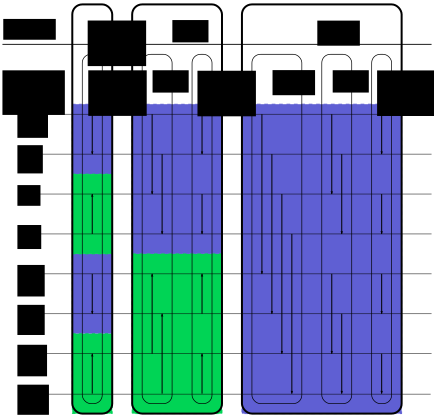
\includegraphics[scale=0.5]{bitonic_sequences.pdf}
    \end{figure}
    \begin{itemize}
      \item
        Siniset lohkot tuottavat nousevan järjestyksen.
      \item
        Vihreät laskevan järjestyksen.
    \end{itemize}
\end{frame}

\begin{frame}{Bitoninen järjestäminen}{Synkronointi}
\begin{columns}
\column{0.2\textwidth}
    \begin{figure}
        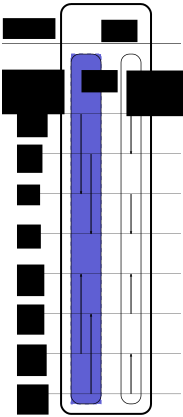
\includegraphics[scale=0.5]{askel.pdf}
    \end{figure}
\column{0.8\textwidth}
    \begin{itemize}
        \item
          Edellisen askeleen kaikkien vertailuoperaatioiden oltava suoritettu ennen seuraavan askeleen aloitusta.
        \item
          Ongelma: vaatii paljon synkronointia ja kommunikointia prosessointiyksiköiden välillä.
        \item
          Ratkaisu: Synkronointia vaativat toiminnot sijoitetaan eri CUDA-ytimiin. Uusi CUDA-ydin käynnistetään aina vasta kun edellisen suoritus on päättynyt.
    \end{itemize}
\end{columns}
\end{frame}

\begin{frame}{Bitoninen järjestäminen}{Naiivi CUDA-toteutus}
\begin{columns}
\column{0.4\textwidth}
    \begin{figure}
        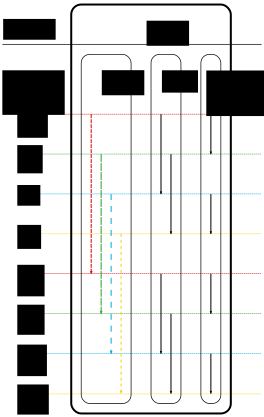
\includegraphics[scale=0.5]{bitonic_naive.pdf}
    \end{figure}
\column{0.6\textwidth}
    \begin{itemize}
        \item Luodaan uusi säie jokaista vertailuoperaatiota varten.
        \item $\frac{n}{2}$ säiettä jokaisessa askeleessa.
        \item Suoritus yksi askel kerrallaan omana CUDA-ytimenään.
        \item Askeleen alussa alkioiden luku globaalista muistista ja askeleen lopussa kirjoitus globaaliin muistiin.
    \end{itemize}
\end{columns}
\end{frame}

\begin{frame}{Bitoninen järjestäminen}{Naiivin CUDA-toteutuksen ongelmia}
    \begin{itemize}
      \item CUDA-ytimiä tarvitaan yhtä monta kuin askeliakin.
      \item Tarvitaan paljon viittauksia globaaliin muistiin ($n$ luku- ja kirjoitusoperaatiota jokaisessa askeleessa).
      \item Viittaukset globaaliin muistiin usein hajanaisia, koska vertailtavat alkiot eivät sijaitse vierekkäin muistissa.
    \end{itemize}
\end{frame}

\begin{frame}{Bitoninen järjestäminen}{Edistyneempi toteutus}
\begin{columns}
\column{0.4\textwidth}
    \begin{figure}
        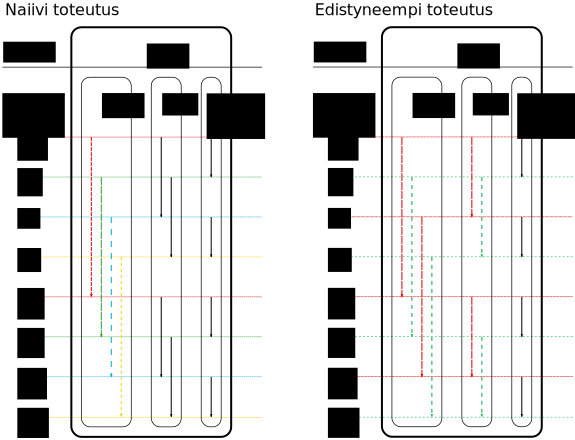
\includegraphics[scale=0.5]{bitonic_advanced.pdf}
    \end{figure}
\column{0.6\textwidth}
    \begin{itemize}
      \item
        Yksi säie prosessoi useita peräkkäisiä vertailuoperaatioita eri askelista.
      \item
        Valitaan vertailuoperaatioita, jotka käsittelevät samaa alkiojoukkoa.
      \item
        Säikeen ulkopuoliset vertailuoperaatiot eivät saa koskea näihin alkioihin.
    \end{itemize}
\end{columns}
\end{frame}

\begin{frame}{Bitoninen järjestäminen}{Edistyneempi toteutus}
\begin{columns}
\column{0.4\textwidth}
    \begin{figure}
        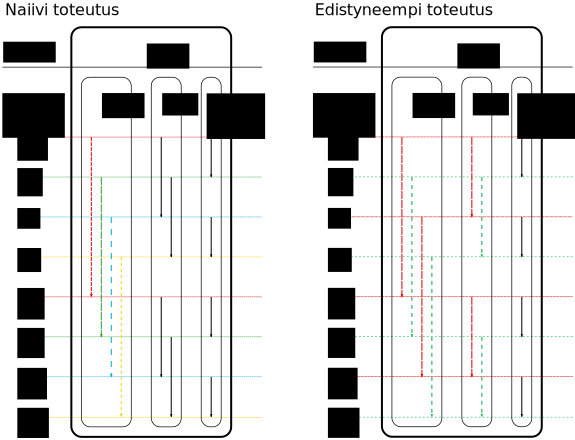
\includegraphics[scale=0.5]{bitonic_advanced.pdf}
    \end{figure}
\column{0.6\textwidth}
    \begin{itemize}
      \item
        Pitemmillä syötteillä voidaan ketjuttaa useampiakin askelia.
      \item
        Mutta: Säikeiden määrää ei haluta vähentää liikaa. (Resurssienkäyttö.)
      \item
        Käytetään yksittäisiä säikeitä säielohkojen sijaan, joten jaettua muistia ei voida hyödyntää. \\ $\Rightarrow$ Ongelmana rekisteritilan rajallisuus.
    \end{itemize}
\end{columns}
\end{frame}

\begin{frame}{Bitoninen järjestäminen}{Kuinka hyödyntää säielohkoja ja jaettua muistia?}
\begin{columns}
\column{0.4\textwidth}
    \begin{figure}
        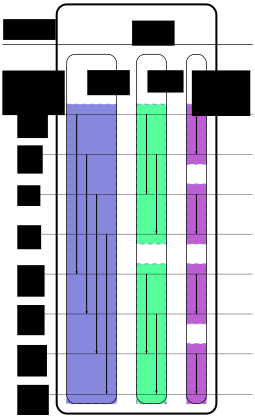
\includegraphics[scale=0.5]{bitonic_subsequences.pdf}
    \end{figure}
\column{0.6\textwidth}
    \begin{itemize}
      \item
        Jokaisessa askeleessa $s$ on $2^s$ alkion alijonoja, jotka käsitellään itsenäisesti.
      \item
        Mikäli tällainen alijono mahtuu kokonaan säielohkon jaettuun muistiin, se voidaan lukea sinne yhdellä yhdistetyllä lukuoperaatiolla.
        % Miksi sanotaan näin? Siis esim. askeleen 3 alkiot voitaisiin kyllä ladata kerralla, mutta askelten 2 ja 1 alijonoilla ei näytä sen jälkeen olevan paljonkaan merkitystä.
      \item
        Tämän jälkeen jako säikeisiin tehdään kuten esitettiin edellä.
      \item
        Tällöin synkronointiin voidaan käyttää nopeaa jaettua muistia.
    \end{itemize}
\end{columns}
\end{frame}

\begin{frame}{Bitoninen järjestäminen}{Yhteenveto}
    \begin{itemize}
      \item
        Ilmeisesti nopein avainten vertailuun perustuvista CUDA-järjestämisalgoritmeista tällä hetkellä.
      \item
        Parhaimmillaan järjestää esim. 32-bittisiä avain-arvo-pareja yli 200 miljoonaa kappaletta sekunnissa.
      \item
        Häviää kuitenkin nopeudessa joillekin radix sort -toteutuksille.
    \end{itemize}
\end{frame}

\end{document}
